\section{Erweitern der Requirements Erkenntnisse}
RE = koordinierte Menge von Aktionen zum Entdecken, Evaluieren, Dokumentieren, Konsolidieren, Überarbeiten von Zielen, Bedingungen, Annahmen, Fähigkeiten die das 'System-to-be' erfüllen sollte um Probleme des 'System-as-is' zu lösen und neue Möglichkeiten zu liefern.

\begin{figure}[h]
	\centering
	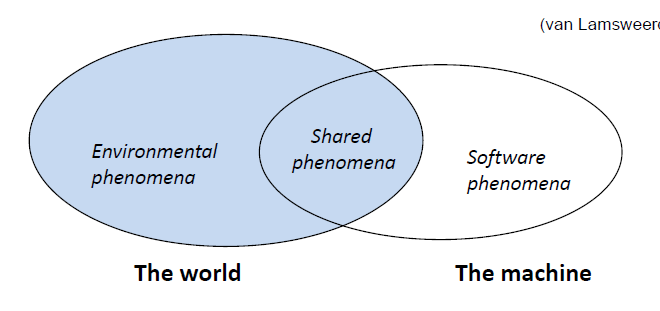
\includegraphics[scale=0.5]{img/re_world.png}
	\caption{Why, What and Who Dimension of RE}
	\label{re_world}
\end{figure}

R beziehen sich auf die Umwelt und betreffen die Maschine nur indirekt.
\begin{itemize}
	\item \textit{System R}: vorgeschrieben Angaben, die das 'System-to-be' u.U. mit anderen System Komponenten, leisten kann
	\item \textit{Software R}: vorgeschriebene Angaben, die \textbf{ausschließlich} das 'System-to-be' leisten kann;
	\begin{itemize}
		\item Domain Properties: Invariante Bedingungen 
		\item Annahmen: müssen erfüllt werden von Umwelt
	\end{itemize}
\end{itemize}

\subsection{Why, What and Who Dimension of RE}
\begin{figure}[h]
	\centering
	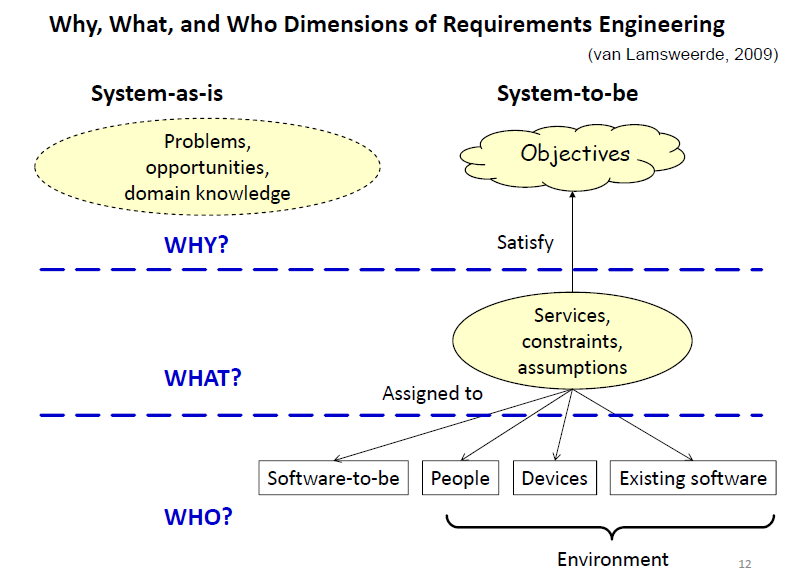
\includegraphics[scale=0.5]{img/re_dimensions.png}
	\caption{Why, What and Who Dimension of RE}
\end{figure}
\begin{itemize}
	\item \textbf{Why-Dimension} kontextbezogene Gründe für ein neues System müssen gegeben werden - in Bezug auf die Ziele, die das neue System erfüllen soll\\
	Ziele anhand der Beschränkungen des aktuellen Systems herausarbeiten\\
	Zielfindung liefert oft Konflikte, da Ziele aus unterschiedlichen Perspektiven def. werden
	
	\item \textbf{What-Dimension} Bestimmen der Dienste, Bedingungen, Annahmen des System-to-be anhand der bestimmten Ziele mit Hilfe von Elicitation Techniken
	
	\item \textbf{Who-Dimension} Bestimmt die Kompetenzen, die notwendig sind um Ziele zu erreichen
\end{itemize}

\subsection{Darstellung der R}
\begin{itemize}
	\item natürliche Sprache für einzelne R nutzen\\
	Verbesserung durch: Strukturierung der R; Regeln für das beschreiben (z.b. Verbot bestimmter Wörter); Redundanzprüfung\\
	Limitierung: nicht zwingend eindeutig; Verknüpfung zw R kann schwer zu ziehen sein
	\item Graphische Notation, die Daten, Funktionen, Verhalten beschreiben
	\item Formale Modelle
	\item Formalisierung R durch\\
	\textit{Designation} = Formale Grundterm (e.g. Prädikat) durch informelle Beschreibung erklären\\
	\textit{Definition} Anhand definierter Termine neue Termine def.; lässt sich besser begründen, aber ist eingeschränkter in der Beschreibung
	
\end{itemize}

\subsection{Zusammenfassung}
\begin{itemize}
	\item R beschreibt Bedingung über ein Phänomen der Umwelt
	\item Beschreibung der R muss die Trennung zw. Maschine und Umwelt respektieren und zw\\
	Umwelteigenschaften, die gegeben sind (indicative) und die von der Maschine geleistet werden (optative)
\end{itemize}
